\section{Kyöpeli}
\begin{figure}[htb]
	\begin{center}
		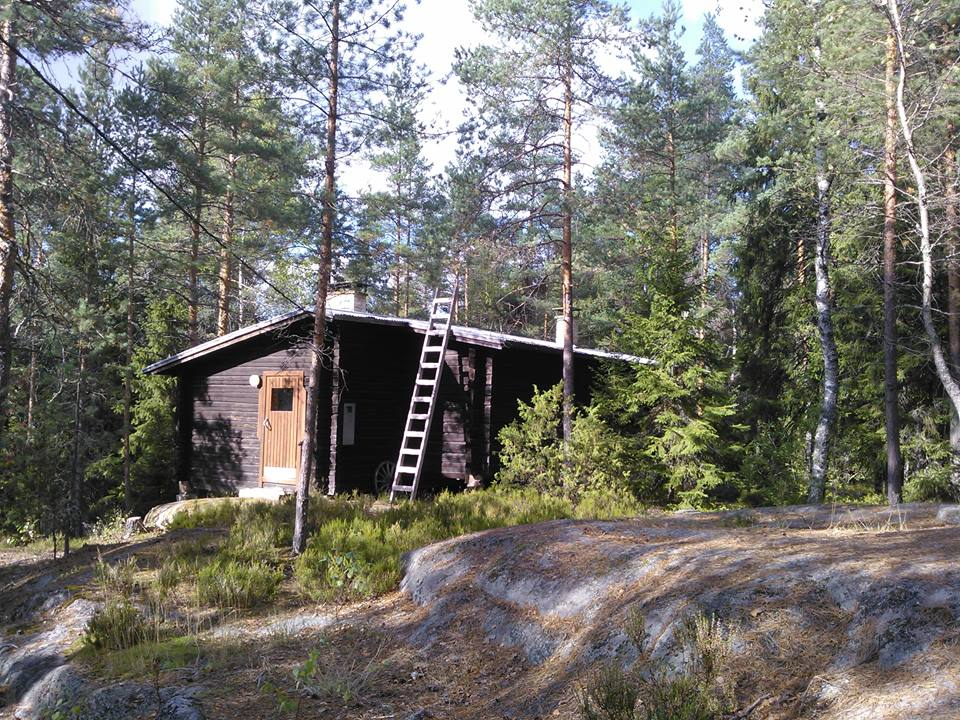
\includegraphics[height=7cm]{kuvat/kyopeli.jpg}
	\end{center}
	\captionsetup{labelformat=empty}
	\caption{\textbf{Lippukunnan kämppä, Kyöpeli.}}
\end{figure}

Lippukunnan pääasiallisena kämppänä toimii osoitteessa Ruuhijärventie 17 sijaitseva Kyöpeli. Kämppään kuuluu laajahko tontti. Kämppää käytetään lippukunnan omiin retkiin ulkopuolelle vuokrauksen lisäksi. Myös lippukunta maksaa omista retkistään vuokraa, jotta kämpän ylläpitoon saadaan riittävästi varoja.\\
\\Kämpän suhteen tehdään läheistä yhteistyötä Paakaupunkiseudun partiolaisten kanssa. Tämä näkyy siten, että lippukunnalla on 1/4-osa käyttöoikeus kaikkiin piirin tarjoamiin palveluihin. Näihin kuuluu sauna, vesikaivo ja jätehuolto.\\
\\Kyöpelillä vietetään joka vuosi talkoot, yleensä Helatorstaina. Tällä toimikaudella talkoissa tehtiin valtavat määrät puutöitä sekä uudet penkit nuotiopaikalle, lisäksi sisätiloissa tehtiin parannustöitä keittiöön.
\newpage
